\documentclass{article}\usepackage[]{graphicx}\usepackage[]{color}
%% maxwidth is the original width if it is less than linewidth
%% otherwise use linewidth (to make sure the graphics do not exceed the margin)
\makeatletter
\def\maxwidth{ %
  \ifdim\Gin@nat@width>\linewidth
    \linewidth
  \else
    \Gin@nat@width
  \fi
}
\makeatother

\definecolor{fgcolor}{rgb}{0.345, 0.345, 0.345}
\newcommand{\hlnum}[1]{\textcolor[rgb]{0.686,0.059,0.569}{#1}}%
\newcommand{\hlstr}[1]{\textcolor[rgb]{0.192,0.494,0.8}{#1}}%
\newcommand{\hlcom}[1]{\textcolor[rgb]{0.678,0.584,0.686}{\textit{#1}}}%
\newcommand{\hlopt}[1]{\textcolor[rgb]{0,0,0}{#1}}%
\newcommand{\hlstd}[1]{\textcolor[rgb]{0.345,0.345,0.345}{#1}}%
\newcommand{\hlkwa}[1]{\textcolor[rgb]{0.161,0.373,0.58}{\textbf{#1}}}%
\newcommand{\hlkwb}[1]{\textcolor[rgb]{0.69,0.353,0.396}{#1}}%
\newcommand{\hlkwc}[1]{\textcolor[rgb]{0.333,0.667,0.333}{#1}}%
\newcommand{\hlkwd}[1]{\textcolor[rgb]{0.737,0.353,0.396}{\textbf{#1}}}%
\let\hlipl\hlkwb

\usepackage{framed}
\makeatletter
\newenvironment{kframe}{%
 \def\at@end@of@kframe{}%
 \ifinner\ifhmode%
  \def\at@end@of@kframe{\end{minipage}}%
  \begin{minipage}{\columnwidth}%
 \fi\fi%
 \def\FrameCommand##1{\hskip\@totalleftmargin \hskip-\fboxsep
 \colorbox{shadecolor}{##1}\hskip-\fboxsep
     % There is no \\@totalrightmargin, so:
     \hskip-\linewidth \hskip-\@totalleftmargin \hskip\columnwidth}%
 \MakeFramed {\advance\hsize-\width
   \@totalleftmargin\z@ \linewidth\hsize
   \@setminipage}}%
 {\par\unskip\endMakeFramed%
 \at@end@of@kframe}
\makeatother

\definecolor{shadecolor}{rgb}{.97, .97, .97}
\definecolor{messagecolor}{rgb}{0, 0, 0}
\definecolor{warningcolor}{rgb}{1, 0, 1}
\definecolor{errorcolor}{rgb}{1, 0, 0}
\newenvironment{knitrout}{}{} % an empty environment to be redefined in TeX

\usepackage{alltt}
\usepackage{Sweave}
\usepackage{float}
\usepackage{graphicx}
\usepackage{tabularx}
\usepackage{siunitx}
\usepackage{mdframed}
\usepackage{natbib}
\bibliographystyle{.//refs/styles/besjournals.bst}
\usepackage[small]{caption}
\setkeys{Gin}{width=0.8\textwidth}
\setlength{\captionmargin}{30pt}
\setlength{\abovecaptionskip}{0pt}
\setlength{\belowcaptionskip}{10pt}
\topmargin -1cm        
\oddsidemargin -0.04cm   
\evensidemargin -0.04cm
\textwidth 16.59cm
\textheight 20.94cm 
%\pagestyle{empty} %comment if want page numbers
\parskip 0pt
\renewcommand{\baselinestretch}{1.75}
\parindent 15pt

\newmdenv[
  topline=true,
  bottomline=true,
  skipabove=\topsep,
  skipbelow=\topsep
]{siderules}
\IfFileExists{upquote.sty}{\usepackage{upquote}}{}
\begin{document}
Daniel Buonaiuto\\
OEB 201\\
November 29, 2017
\section*{\textbf{Is Bud Size a Predictor of Phenology in Temperate Woody Plants?}}


\section*{Project Aim}
\par Phenology, the study of organisms' annual life cycle events, has received increased attention in the science of the past decades as phenological changes have appeared as one of the most apparent hallmarks of a changing climate \citep{Menzel2006}. Temperature and photoperiod have been identified as the major drivers of variation in phenology for temperate zone plants \citep{Forrest2010}, but as our understanding of the implications of changing phenology grows, it is critical to explore other drivers that serve to fine-tune phenological expression in organisms. It is possible that both intra-specific variation in phenology could be linked with other physiological differences between individuals. One promising physiological trait for fine-tuning predictions of the timing of budburst in temperate woody plants is the size of their winter buds. It would be expected that larger buds would burst earlier than their small counterparts, assuming that larger buds are a sign of greater initial investment in leaf tissue.The paper below details an experiment designed to test this hypothesis. In the following section I will discuss the methods of study, with an emphasis on the statistical approach I used. I will then discuss preliminary results of the analysis and make recommendations for a more complete approach.
\section*{Methods}
\subsection*{The data}
\par In January of 2015, 40 cm cuttings from 27 temperate woody plant species were collected from two sites in Eastern North America (Harvard Forest, Massachusetts, USA and Saint Hippolyte, Quebec, Canada). The collection included 6 replicates per species, with buds per replicate varying, resulting in a data set of 6,467 rows with data at the individual bud level. For each cutting, bud length and volume were measured with calipers. For many individuals, buds were massed, fixed in a formalin-ethanol solution and dissected with the intention of evaluating other bud characteristics that might affect timing of bud burst such as bud determinism and structure, but these procedures are beyond the scope of this analysis and will not be discussed in detail. Bud width and length were used to calculate bud volume using the equation:

V=\pi(r^2)(h/3)

where r is one half of the bud width and h is bud length. It should be noted that bud measurements were taken over a ~3 month period, and most individuals from Harvard Forest measured before those from Saint Hippolyte. Because it is biologically possible that buds would grow between the time when they were cut from the tree and when they were measured, this measurement pattern produces a potential temporal bias in these data (see figure 1). Much of the statistical analysis presented below will detail the development of the model used to correct for this bias.

\subsection*{Statistical Analysis}
\par To correct for the temporal bias in the data, I developed a model predicting how much bud volume could change per unit time. This model was built from a subset of the full data set which included some repeat measurements from Harvard Forest, was restricted to include only measurements Harvard Forest measurement recorded in a 30 day window, and the few Saint Hippolyte measurements recorded at the same time. Since the data were unbalanced at the species level and it is likely that species would differ considerably both in their absolute bud volume and rate of change, I used a Bayesian multilevel, varying slope, varying intercept at the species level model to predict bud volume and a function of day of year of measurement. All computing was done using R statistical software, and models were specified using the package rstanarm\citep{Stan2016}. The model is specified below:

y_[_i_]=$\alpha$_[_j_]_[_i_}$\beta$_[_j_]X_[_i_]+ e\\

where alpha is a species specific intercept and beta is a species specific coefficient for the predictor day of measurement, represented here by X. First, to test this model's ability to return true values, I simulated a data set of bud volumes for 20 species with 100 observations each, and simulated measurements over a time span of 30 days. In this data set. I set the true global intercept of bud volume to be 8 and effect of date of measurement to be 0.1, and let these values vary by species. The model fit was evaluated with posterior predictive checks (see supplement). \\
Once the model returned the proper values for the simulated data (see next section for more details), I applied the model to the real data set. To fit the modeling frame work, I transformed bud volume distribution to normal using a logarithmic transformation. \par Just as with the simulated data, the model's accuracy was evaluated using posterior predictive checks (see supplement).\\
The model output a species specific coefficient for the effect of day of measurement on bud volume, and these coefficients were used to produce a true bud volume estimate for the full data set, which can be best described as the expected bud volume if all individuals had been measured on the day 40 of the year. The formula used for the bias correct is specified below:

True_b_u_d_v_o_l_u_m_e = measured_b_u_d_v_o_l_u_m_e - $\beta$_[_i_]*(measured_d_a_y- 40)

where $\beta$ is the species specific model coefficient for day of measurement, representing the expected change in volume per day.
\subsection*{Modeling phenology as a function of bud volume}
\par As stated in the introduction, the ultimate goal of this project was to evaluate the role that resting bud size plays in fin-tuning phenological event dates. The following section details the beginning states of developing such a model. To this aim, I obtained phenological event information from another experiment that used cuttings from the same parent plants that were used to create the bud measurement data. In this experiment, cuttings were grown in growth chambers under varying winter chilling temperature, photoperiod and spirng warming temperature regimes, and phenological responses (days to budburst) were observed, resulting in 2136 rows of data recorded at the twig level.
\par As a first pass, for each individual parent, I calculated the mean true bud volume (data set I) and mean phenological response across all experimental treatments (data set II). I built a preliminary, multi level, varying slope and intercept at the species level model to evaluate the possible influence of physiological predictors such as bud volume and twig diameter on phenological rank. The model is specified below:

y[i] = $\alpha$_[_j]_[_i_] +$\beta$_1_[_j_]X_[_i_]+$\beta$_2_[j}Z_[_i_]+ e

where predictors X and Z are mean bud volume and stem diameter respectively, $\alpha$ is the species specific intercept and the $\beta's$ are the species specific coefficients for bud volume and stem diameter respectively.
Finally, it should be noted that I did not heavily interpret this model and do not feel the results are robust. Rather, these model results should be view as a step in the process of creating a more robust model to address this question in the future.
\section*{Results and Discussion}
\subsection*{Bias Correction}
\par The bias correction model, when run on simulated data returned the true values of the parameters (see figure 2, 3).
The model, when applied to the real data, predicts a non-detectable global effect of date of measurement on bud volume. There is high predictive uncertainty associated with this model (sigma= 4.1 see figure 4) and small effect size estimates which likely contribute to this result. Because I expect there to be substantial differences between species, the global intercept and coefficient estimates are not of high values in this analysis. When viewing the species specific coefficients for day of measurement (see figure 5), the effect sizes are all very small, however, it is important to note that these estimates represent change in bud volume per day, so for example, the .017 effect size of \textit{Acer rubrum} would mean that a bud measured 90 days after abother, may have grown 1.53 cubic milimeters in that time, which would introduce significant bias if measurement day was not account for.
\par Most species' 95 percent credible intervals were overlapping zero. For such species, there is high uncertainty that and change in bud volume takes place overtime, and the model indicates that the temporal bias is not relevant. Some species, such as \textit{Quercus alba}, \textit{Acer saccharum}, \textit{Populus grandidentata} and \textit{Spirea alba} have negative estimated effect sizes and credible intervals that do not overlap zero. This result fails to support my original hypothesis. While it is possible that bud volume may decrease with time if, for example buds become more desiccated over time, or lose protective structures over the course of the season, the effect of shrinking buds with time runs counter to my biological hypothesis and the observation that buds swell as they approach budburst. Several other species, \textit{Acer pensylvanicum}, \textit{Acer rubrum}, \textit{Fagus grandifolia} and \textit{Lonicera canadensis} show the biologically expected trend, with positive coefficient estimates and credible intervals that do not overlap zero. Because the sources of bias was based on the expectation that buds grow over time, it may be tempting to only perform bias correction on the 4 species that fit the expected pattern, but with high predictive uncertainty and no mechanisms for conclusively saying that the positive coefficients are the result of a biological mechanism an the negative coefficients are a statistical artifact, I determined to use all coefficient values, and project adjusted bud volumes for each individual(see figure 6).
\subsection*{Phenological predictions}
\par As mentioned above in the methods section, no serious conclusion should be drawn from this model, but it should rather be considered a building block for future analysis. Global coefficients estimates for the effect sizes of both stem diameter and bud volume are negative, which is in line with my hypothesis that larger buds (and thicker stems) are more primed for budburst and can burst earlier. Larger buds may indicated more advanced development, and thicker stems larger reservoirs of stored nutrients that can be utilized by developing leaves. However, for both parameters, the 95 credible intervals overlap zero, so it can be determined there is considerable uncertainty in these predictions. As seen in the posterior checks (see supplement), the model tends to miss a dip and spike in the data on the higher side of the distribution and overestimate phenological response in this region.
\par I will now wrap up this section by proposing strategies that could be used to improve this model moving forward. This model does not acknowledge many factors that may be important biologically in influencing budburst timing. Adding predictors such as site, tree dbh (as a proxy for age), location of bud on the twig, or other physiological predictors might serve to absorb some of the uncertainty. A sound analysis of these data also calls for a more sophisticated hierarchical model, which would allow for the predictors (for example bud volume) to be evaluated on the individual bud level and the response (days to budburst) at the twig level rather than averaging as I did in this preliminary analysis. This would allow for the treatment effect to be maintained in the model, which would be expected to be a major source of variation.
\par In conclusion, in this project I have developed a fairy reliable  estimation of true bud volume from a temporally biased data set. An improvement to this method would be to take more repeat measures over a similar time window, so changes in size could be more accurately observed rather than inferred. I also began to develop a model to determine if bud volume and stem diameter is a predictor for phenological rank within species, and laid out possible next steps for building a more robust model.

\bibliography{.//refs/statsbib}

\section*{Figures}

\begin{figure}[h!]
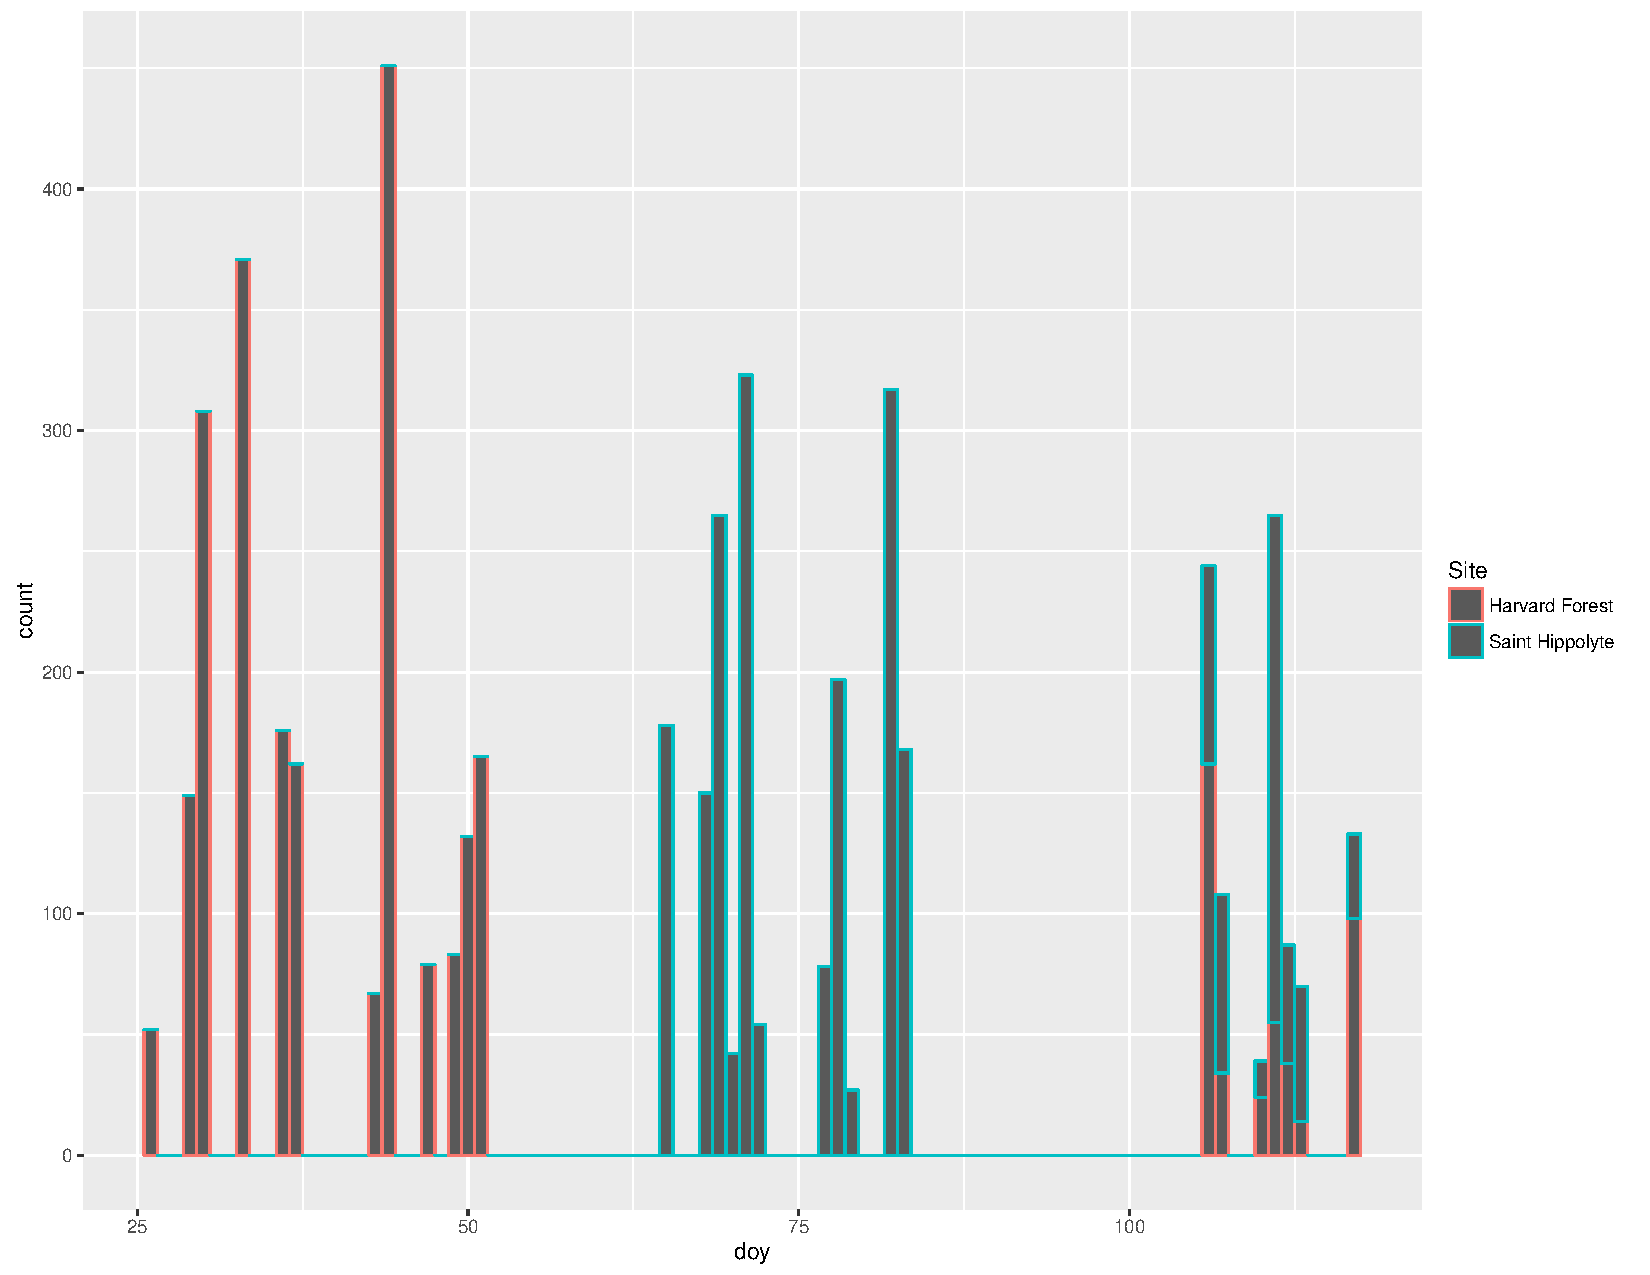
\includegraphics[width=6cm, height=6cm]{temp_bias_fig.pdf}\\
\caption{Measurement days of buds colored by site. Twigs from the different site were measured non-randomly, producing a temporal bias}
\end{figure}


\begin{figure}
\begin{tabular}{c|c|c|c|c|c}
 & Actual & Median& MAD SD & CI_5 & CI_95\\
\hline
Intercept & 8 & 8.3 & 1.4 & 5.99 & 10.67\\
\hline
doy & 0.1 &0.1 & 0.0 & 0.0337 & 0.159\\
\hline
sigma & 4 & 4.1 & 0.1 &  & \\
\hline
\end{tabular}
\caption{real and model predicted effects for simulated data with standard deviation and 95 percent credible intervals}
\end{figure}

\begin{figure}[h!]
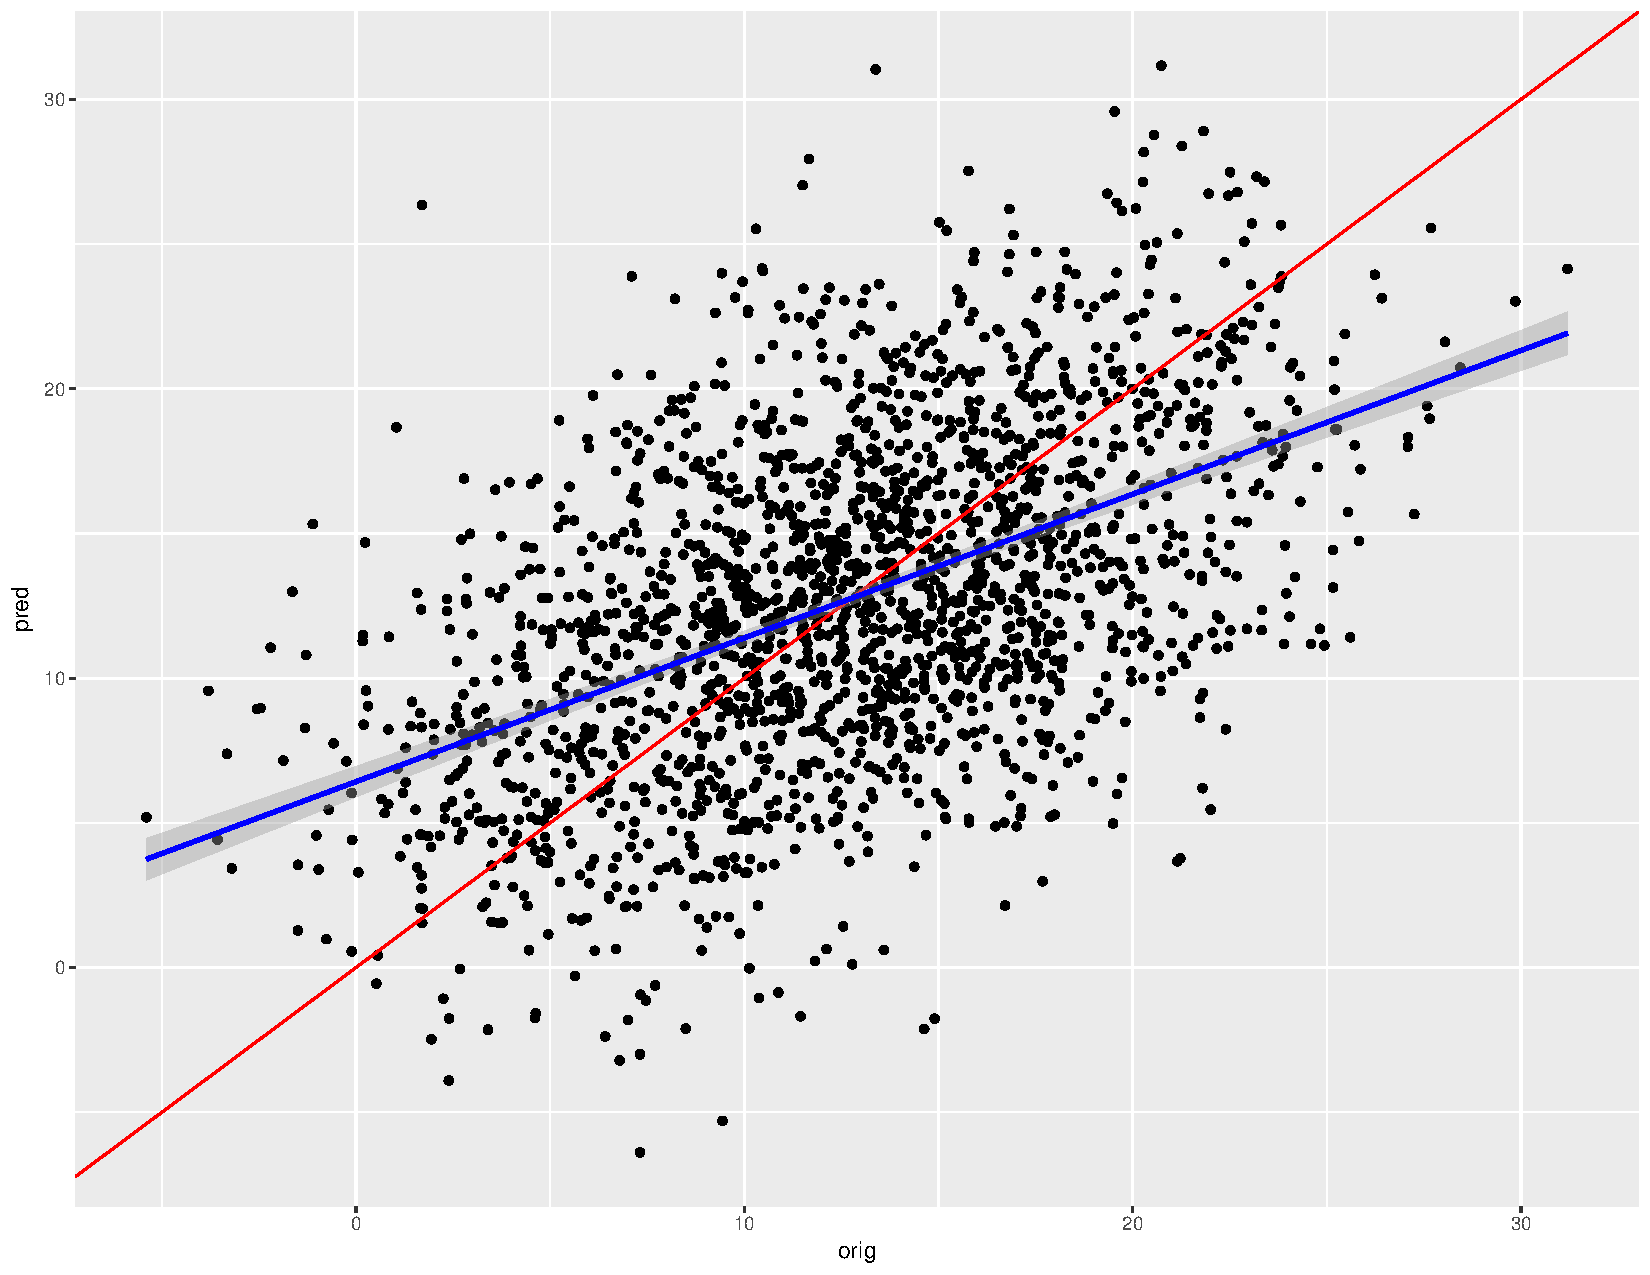
\includegraphics[width=6cm, height=6cm]{fake_predvsorig_final.pdf}\\
\caption{Predicted vs. original values for fake data. The red line represents the 1:1 line which would represent perfect prediction. The blue line is the actual slope, demonstration some deviation}
\end{figure}

\begin{figure}
\begin{tabular}{c|c|c|c|c}
& Median& MAD_SD & CI5 & CI95\\
\hline
Intercept& 0.3 & 0.3 & -1.8e-01 & 0.82\\
\hline
doy &0.0 & 0.0 & -1.03e-03  &0.008 \\
\hline
sigma & 4.1 & 0.0 &1.4042e+00 & 1.45046 \\
\hline
\end{tabular}
\caption{Global intercept and coefficient estimates for bias correction model}
\end{figure}

\begin{figure}[h!]
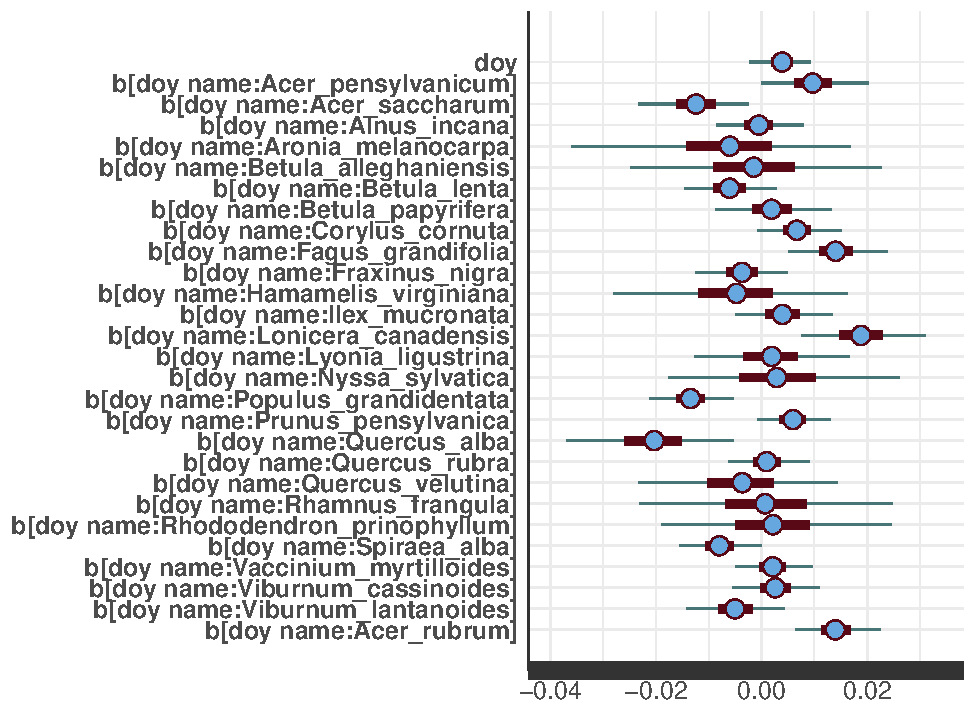
\includegraphics[width=15cm, height=10cm]{shinstan_multiparam.pdf}\\
\caption{The mean effect sizes estimates and 50 and 95 credible intervals of day of measurement on each of the 27 study species from the model bvol ~ doy + (doy | sp)}
\end{figure}

\begin{figure}[h!]
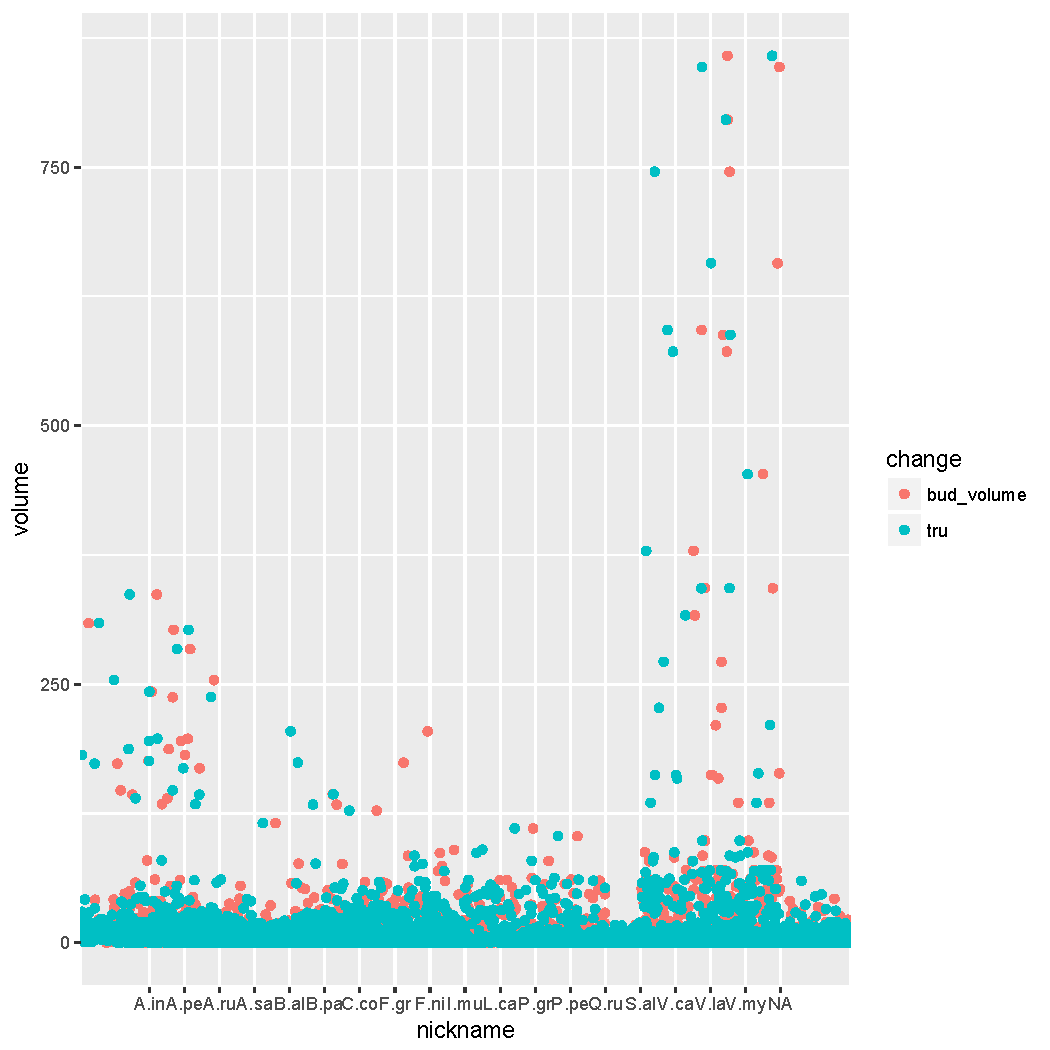
\includegraphics[width=15cm, height=10cm]{tru_vs_measured_partial.pdf}\\
\caption{Temporal bias correction. Blue dots demonstrate the corrected values against the original (red). The plot has been horizontally jittered for better viewing}
\end{figure}

\begin{figure}[h!]
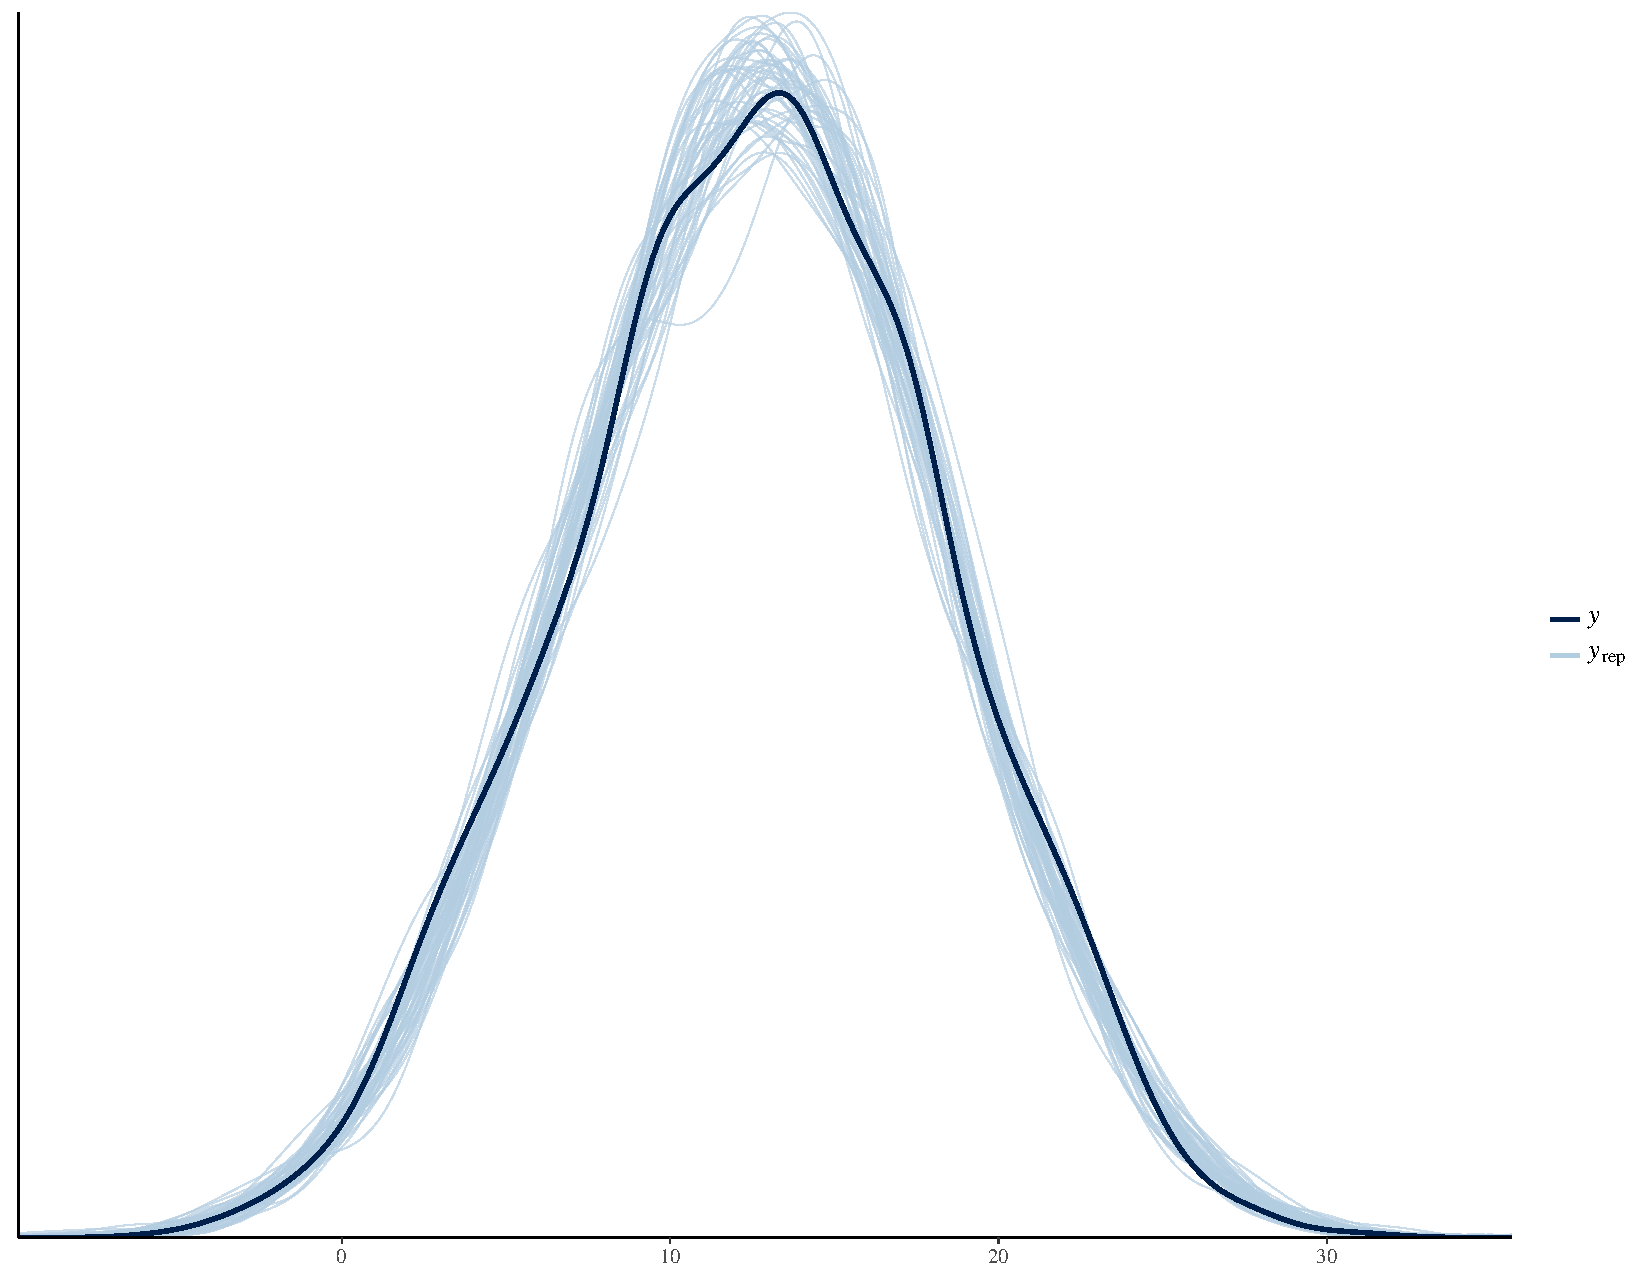
\includegraphics[width=5cm, height=5cm]{fake_data_pp_check_final.pdf}\\
\caption{SUPPLIMENT: Posterior predictive checks for model bvol ~ doy + (doy | sp) on fake data}
\end{figure}

\begin{figure}[h!]
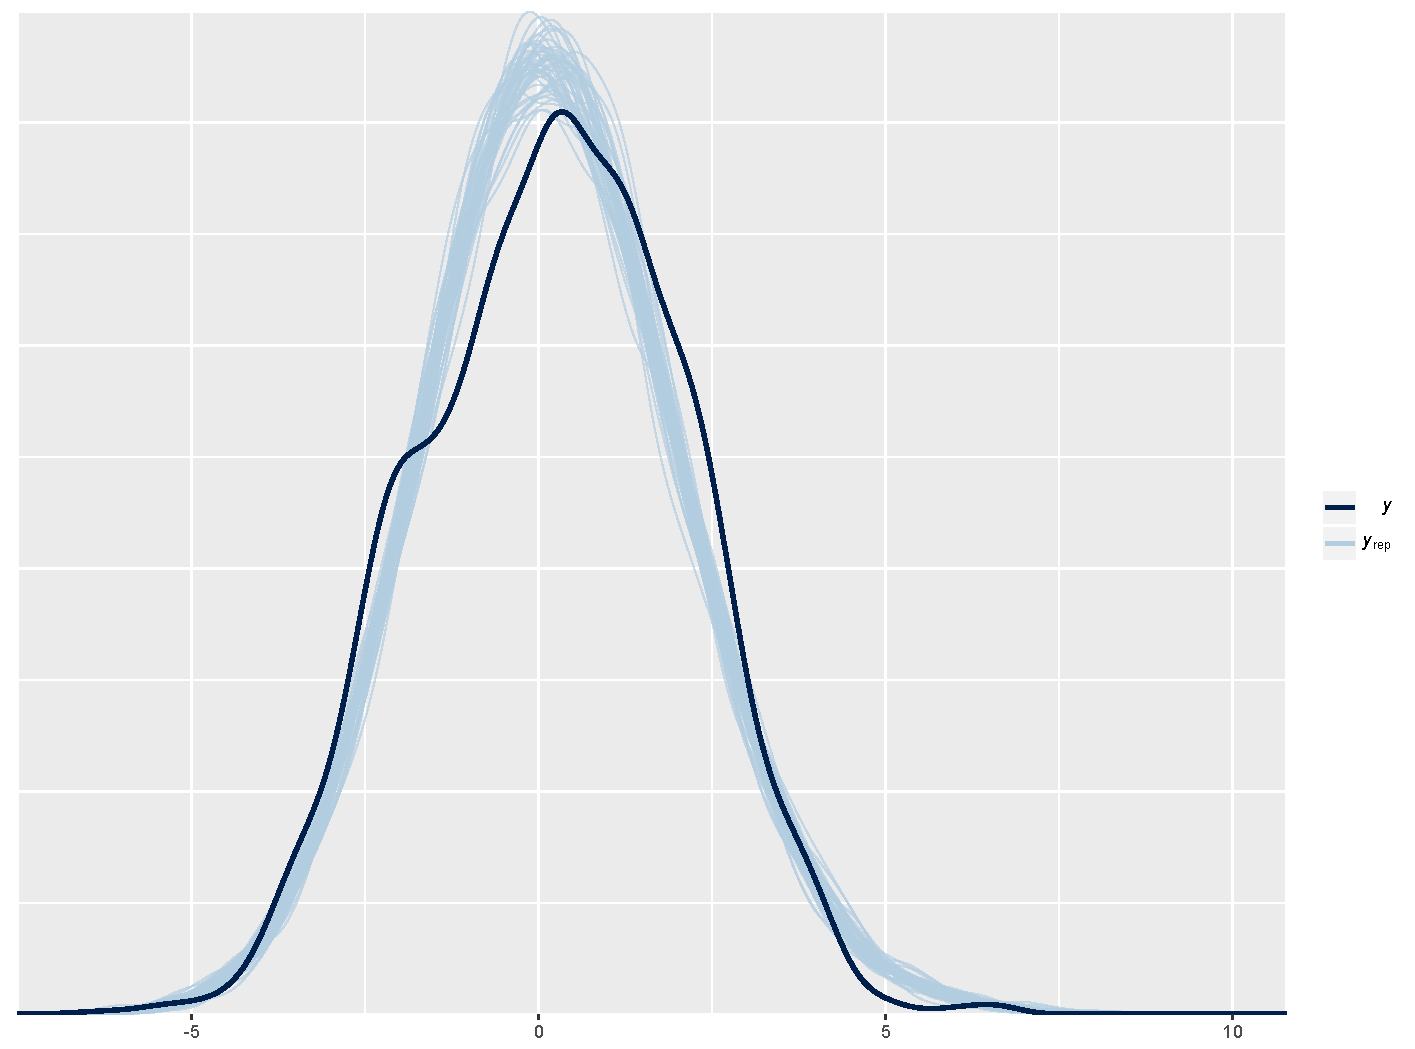
\includegraphics[width=5cm, height=5cm]{pp_check_log_real.pdf}\\
\caption{SUPPLIMENT: Posterior predictive checks for model bvol ~ doy + (doy | sp) on real data}
\end{figure}

\begin{figure}[h!]
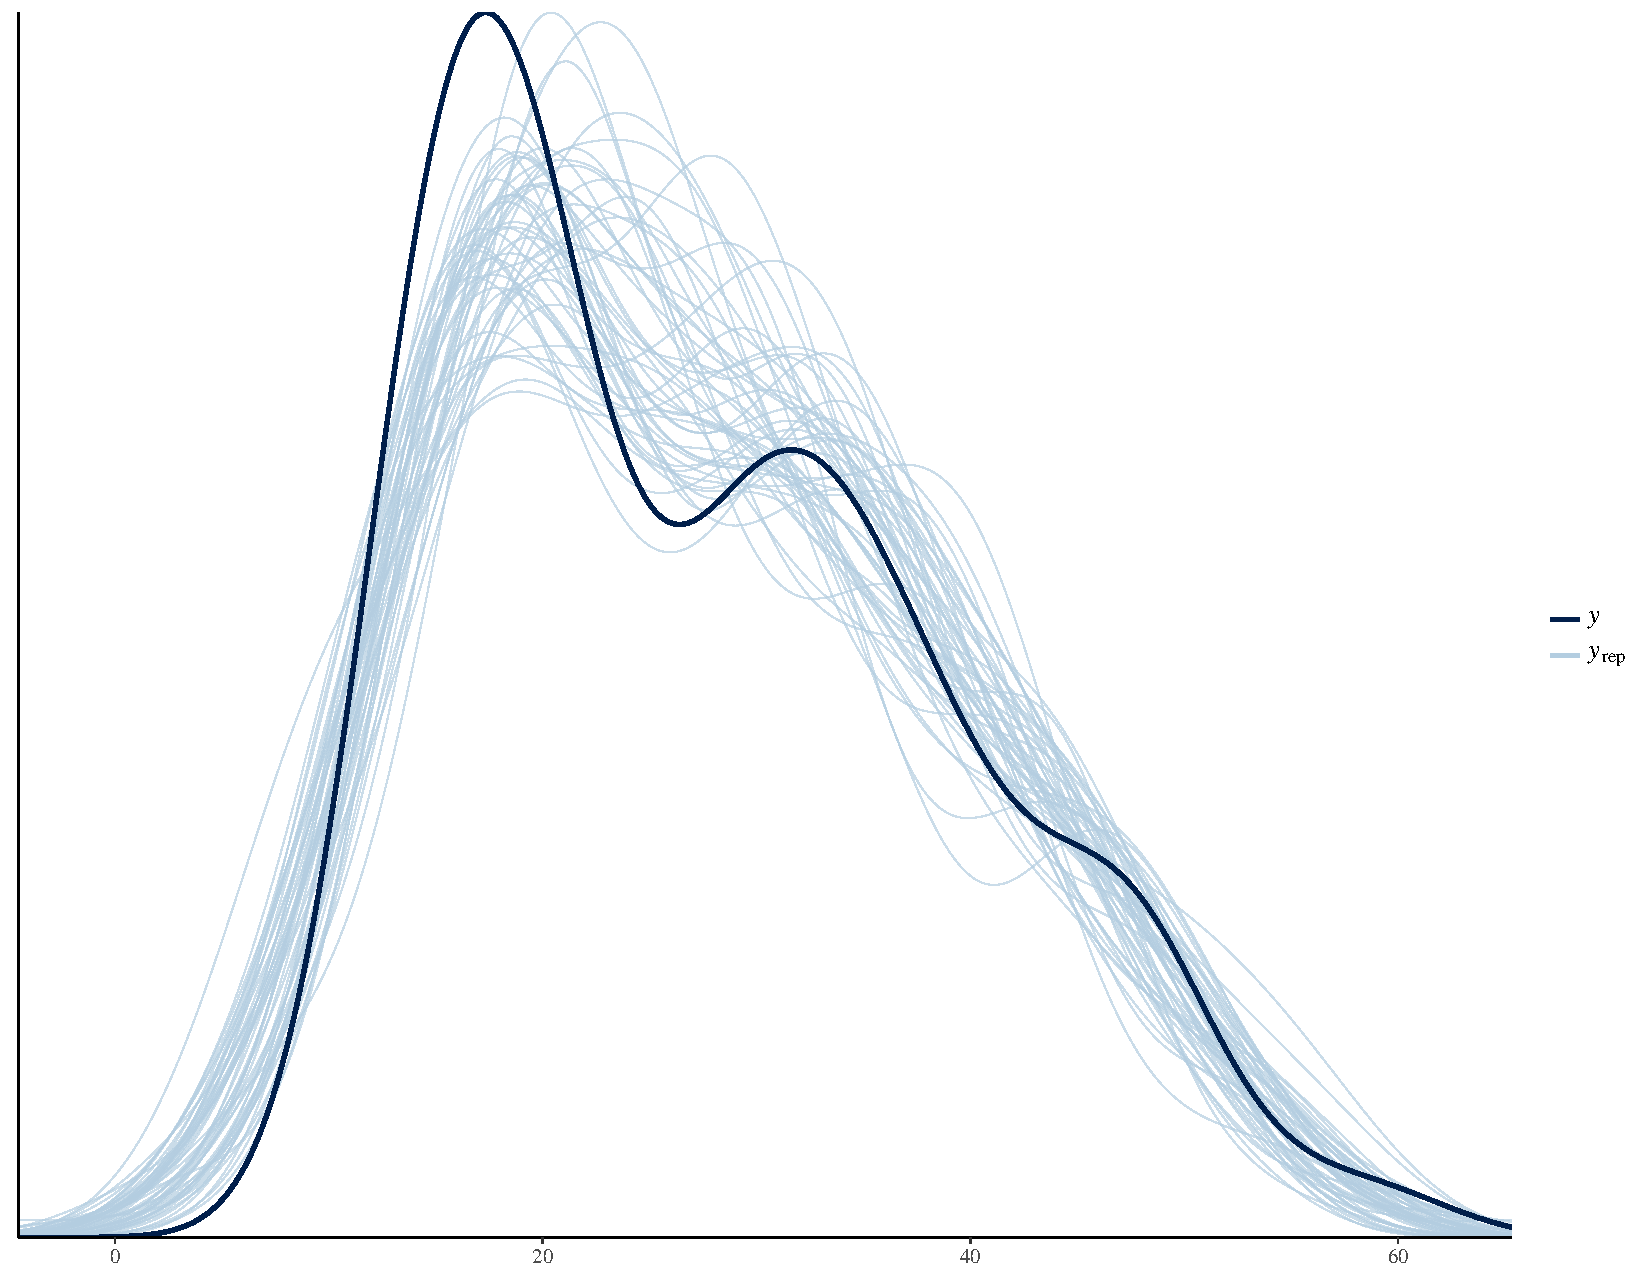
\includegraphics[width=5cm, height=5cm]{moodle_ppcheck.pdf}\\
\caption{SUPPLIMENT: Posterior predictive check for exploratory model meanbday ~ meanstemdiam + meanbvol + (meanstemdiam + meanbvol | SP)}
\end{figure}

\end{document}
